\input{preamble.tex}

\title{Лабораторная работа № 8. \\ Адресация IPv4 и IPv6. Настройка маршрутизации}
\author{Данила Стариков \\ НПИбд-02-22}
\institute{Российский университет дружбы народов имени Патриса Лумумбы}
\date{2024}

\begin{document}

\frame{\titlepage}

\begin{frame}
  \frametitle{Цель работы}
  \begin{itemize}
  \item Изучение принципов маршрутизации в IPv4- и IPv6-сетях и принципов настройки сетевого оборудования
  \end{itemize}
\end{frame}


\begin{frame}
  \frametitle{Настройка динамической маршрутизации в сетях IPv4 и IPv6}
  \begin{table}[]
    \centering
    \caption{Таблица адресов сетей}
    \label{tab1}
    \begin{tabular}{|l|l|l|}
      \hline
      Устройства    & Сеть IPv4    & Сеть IPv6    \\ \hline
      PC1 – gw-01   & 10.0.10.0/24 & 2001:10::/64 \\ \hline
      PC2 – gw-03   & 10.0.11.0/24 & 2001:11::/64 \\ \hline
      gw-01 – gw-02 & 10.0.1.0/24  & 2001:1::/64  \\ \hline
      gw-02 – gw-03 & 10.0.2.0/24  & 2001:2::/64  \\ \hline
      gw-03 – gw-04 & 10.0.3.0/24  & 2001:3::/64  \\ \hline
      gw-04 – gw-01 & 10.0.4.0/24  & 2001:4::/64  \\ \hline
    \end{tabular}
  \end{table}
\end{frame}

\begin{frame}
  \frametitle{Настройка динамической маршрутизации в сетях IPv4 и IPv6}
  \centering
  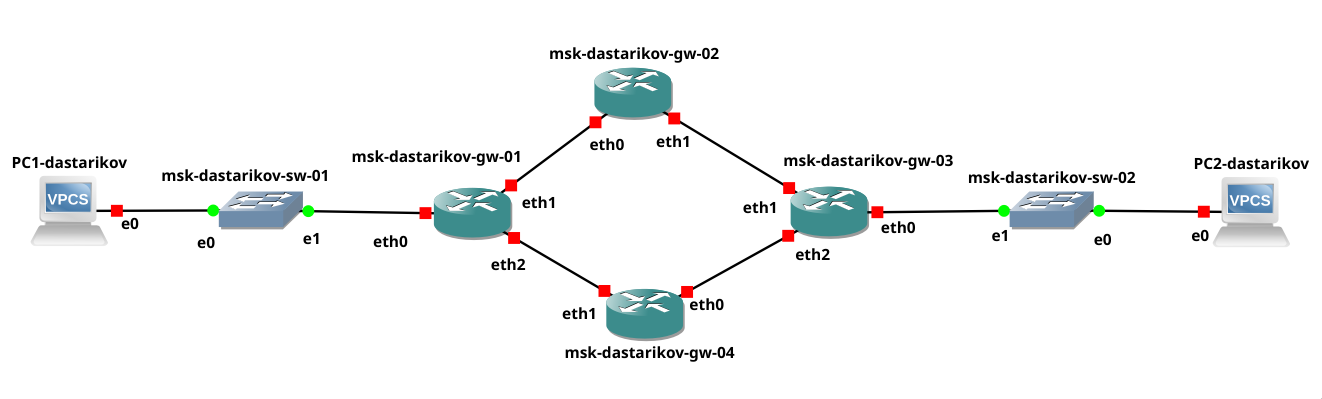
\includegraphics[width=0.8\textwidth]{../images/image00.png}
  \captionof{figure}{Топология сети.}
\end{frame}

\begin{frame}
  \frametitle{Настройка динамической маршрутизации в сетях IPv4 и IPv6}
  \centering
  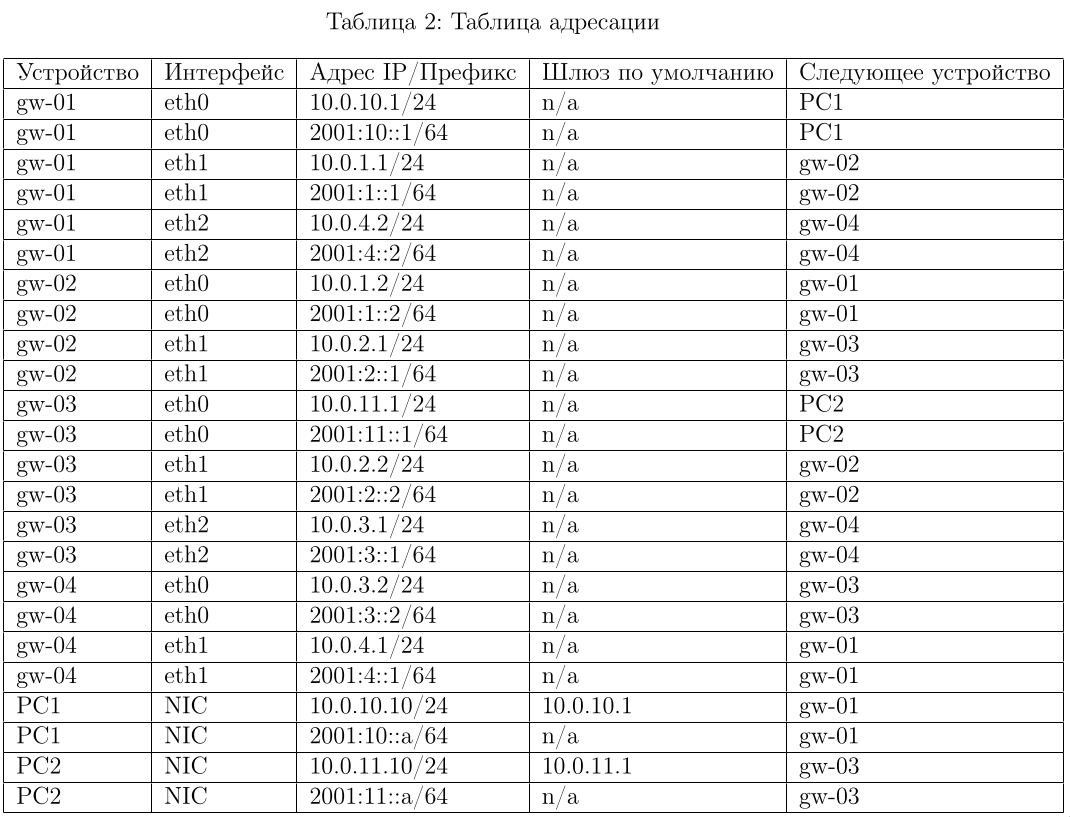
\includegraphics[width=0.8\textwidth]{../images/image_tab2.png}
\end{frame}

\begin{frame}
  \frametitle{Настройка динамической маршрутизации в сетях IPv4 и IPv6}
      \centering
  
\includegraphics[width=0.8\textwidth]{../images/image21.png}
  \captionof{figure}{Настройка протокола RIP на маршрутизатору \texttt{gw-01}.}
\end{frame}

\begin{frame}
  \frametitle{Настройка динамической маршрутизации в сетях IPv4 и IPv6}
  \centering
  
\includegraphics[width=0.8\textwidth]{../images/image22.png}
  \captionof{figure}{Настройка протокола RIP на маршрутизатору \texttt{gw-02}.}
\end{frame}

\begin{frame}
  \frametitle{Настройка динамической маршрутизации в сетях IPv4 и IPv6}
  \centering
  
\includegraphics[width=0.8\textwidth]{../images/image23.png}
  \captionof{figure}{Настройка протокола RIP на маршрутизатору \texttt{gw-03}.}
\end{frame}

\begin{frame}
  \frametitle{Настройка динамической маршрутизации в сетях IPv4 и IPv6}
  \centering
  
\includegraphics[width=0.8\textwidth]{../images/image24.png}
  \captionof{figure}{Настройка протокола RIP на маршрутизатору \texttt{gw-04}.}
\end{frame}

\begin{frame}
  \frametitle{Настройка динамической маршрутизации в сетях IPv4 и IPv6}
      \centering
      
\includegraphics[width=0.8\textwidth]{../images/image25.png}
      \captionof{figure}{Просмотр настроек маршрутизации по RIP.}
\end{frame}

\begin{frame}
  \frametitle{Настройка динамической маршрутизации в сетях IPv4 и IPv6}
      \centering
      
\includegraphics[width=0.8\textwidth]{../images/image26.png}
      \captionof{figure}{Просмотр настроек маршрутизации по RIP.}
\end{frame}

\begin{frame}
  \frametitle{Настройка динамической маршрутизации в сетях IPv4 и IPv6}
      \centering
      
\includegraphics[width=0.8\textwidth]{../images/image27.png}
      \captionof{figure}{Просмотр настроек маршрутизации по RIP.}
\end{frame}

\begin{frame}
  \frametitle{Настройка динамической маршрутизации в сетях IPv4 и IPv6}
        \centering
        
\includegraphics[width=0.8\textwidth]{../images/image28.png}
        \captionof{figure}{Отправка эхо-запроса с PC1 к PC2.}
\end{frame}

\begin{frame}
  \frametitle{Настройка динамической маршрутизации в сетях IPv4 и IPv6}
        \centering
        
\includegraphics[width=0.8\textwidth]{../images/image30.png}
        \captionof{figure}{Отключение на маршрутизаторе \texttt{msk-dastarikov-gw-02} интерфейса \texttt{eth0}.}
\end{frame}

\begin{frame}
  \frametitle{Настройка динамической маршрутизации в сетях IPv4 и IPv6}
        \centering
        
\includegraphics[width=0.8\textwidth]{../images/image31.png}
        \captionof{figure}{Просмотр метрики RIP после сразу отключения маршрутизатора.}
\end{frame}

\begin{frame}
  \frametitle{Настройка динамической маршрутизации в сетях IPv4 и IPv6}
        \centering
        
\includegraphics[width=0.8\textwidth]{../images/image32.png}
        \captionof{figure}{Отправка эхо-запроса с PC1 к PC2 по новому маршруту.}
\end{frame}

\begin{frame}
  \frametitle{Настройка динамической маршрутизации в сетях IPv4 и IPv6}
        \centering
        
\includegraphics[width=0.8\textwidth]{../images/image33.png}
        \captionof{figure}{Просмотр метрики RIP после восстановления маршрута сразу отключения.}
\end{frame}

\begin{frame}
  \frametitle{Настройка динамической маршрутизации в сетях IPv4 и IPv6}
      \centering
      
\includegraphics[width=0.8\textwidth]{../images/image34.png}
      \captionof{figure}{Настройка протокола RIPng на маршрутизатору \texttt{gw-01}.}
\end{frame}

\begin{frame}
  \frametitle{Настройка динамической маршрутизации в сетях IPv4 и IPv6}
      \centering
      
\includegraphics[width=0.8\textwidth]{../images/image35.png}
      \captionof{figure}{Настройка протокола RIPng на маршрутизатору \texttt{gw-02}.}
\end{frame}

\begin{frame}
  \frametitle{Настройка динамической маршрутизации в сетях IPv4 и IPv6}
      \centering
      
\includegraphics[width=0.8\textwidth]{../images/image36.png}
      \captionof{figure}{Настройка протокола RIPng на маршрутизатору \texttt{gw-03}.}
\end{frame}

\begin{frame}
  \frametitle{Настройка динамической маршрутизации в сетях IPv4 и IPv6}
      \centering
      
\includegraphics[width=0.8\textwidth]{../images/image37.png}
      \captionof{figure}{Настройка протокола RIPng на маршрутизатору \texttt{gw-04}.}
\end{frame}

\begin{frame}
  \frametitle{Настройка динамической маршрутизации в сетях IPv4 и IPv6}
        \centering
        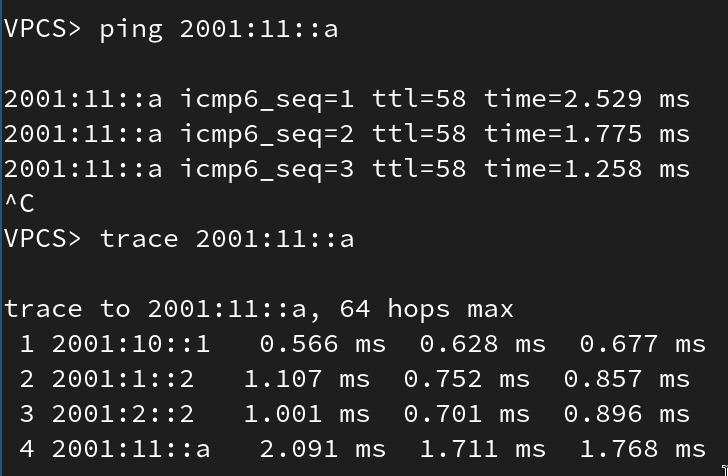
\includegraphics[width=0.8\textwidth]{../images/image38.png}
        \captionof{figure}{Отправка эхо-запроса с PC1 к PC2.}
\end{frame}

\begin{frame}
  \frametitle{Настройка динамической маршрутизации в сетях IPv4 и IPv6}
        \centering
        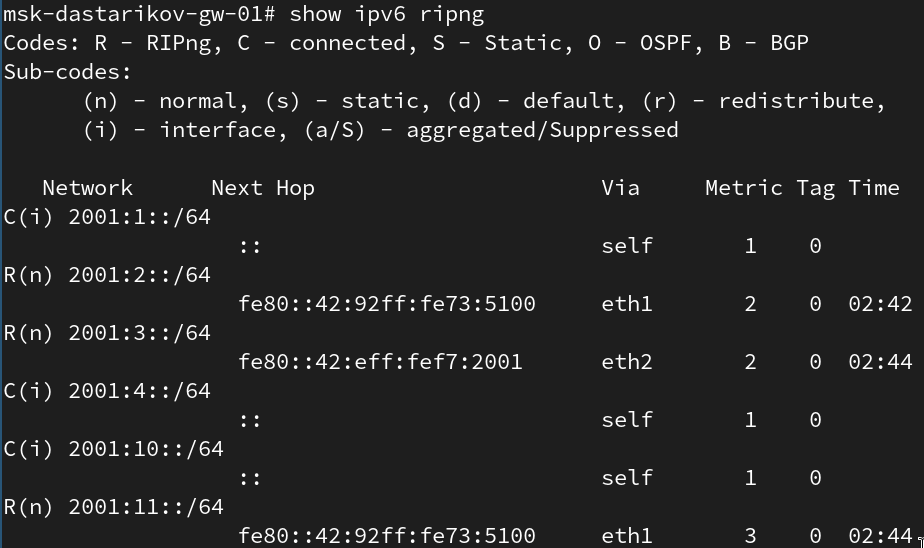
\includegraphics[width=0.8\textwidth]{../images/image39.png}
        \captionof{figure}{Проверка метрики протокола RIPng.}
\end{frame}

\begin{frame}
  \frametitle{Настройка динамической маршрутизации в сетях IPv4 и IPv6}
        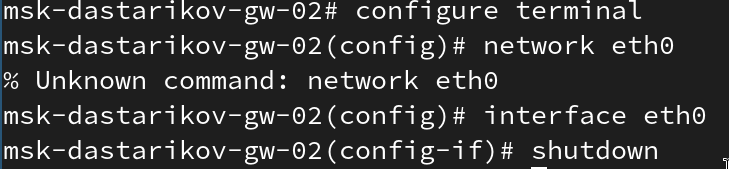
\includegraphics[width=0.8\textwidth]{../images/image40.png}
        \captionof{figure}{Отключение на маршрутизаторе \texttt{msk-dastarikov-gw-02} интерфейса \texttt{eth0}.}
\end{frame}

\begin{frame}
  \frametitle{Настройка динамической маршрутизации в сетях IPv4 и IPv6}
      \centering
      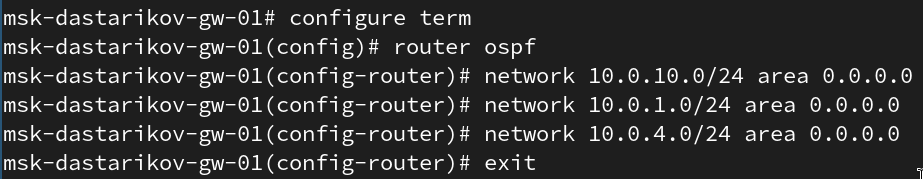
\includegraphics[width=0.8\textwidth]{../images/image41.png}
      \captionof{figure}{Настройка протокола OSPF на маршрутизатору \texttt{gw-01}.}
\end{frame}

\begin{frame}
  \frametitle{Настройка динамической маршрутизации в сетях IPv4 и IPv6}
      \centering
      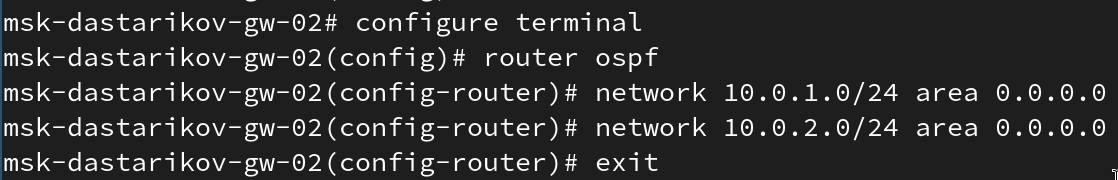
\includegraphics[width=0.8\textwidth]{../images/image42.png}
      \captionof{figure}{Настройка протокола OSPF на маршрутизатору \texttt{gw-02}.}
\end{frame}

\begin{frame}
  \frametitle{Настройка динамической маршрутизации в сетях IPv4 и IPv6}
      \centering
      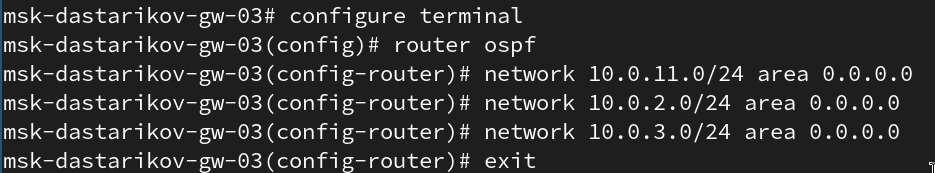
\includegraphics[width=0.8\textwidth]{../images/image43.png}
      \captionof{figure}{Настройка протокола OSPF на маршрутизатору \texttt{gw-03}.}
\end{frame}

\begin{frame}
  \frametitle{Настройка динамической маршрутизации в сетях IPv4 и IPv6}
      \centering
      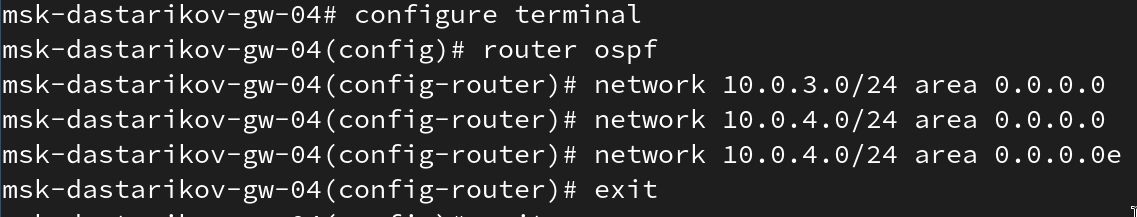
\includegraphics[width=0.8\textwidth]{../images/image44.png}
      \captionof{figure}{Настройка протокола OSPF на маршрутизатору \texttt{gw-04}.}
\end{frame}

\begin{frame}
  \frametitle{Настройка динамической маршрутизации в сетях IPv4 и IPv6}
      \centering
      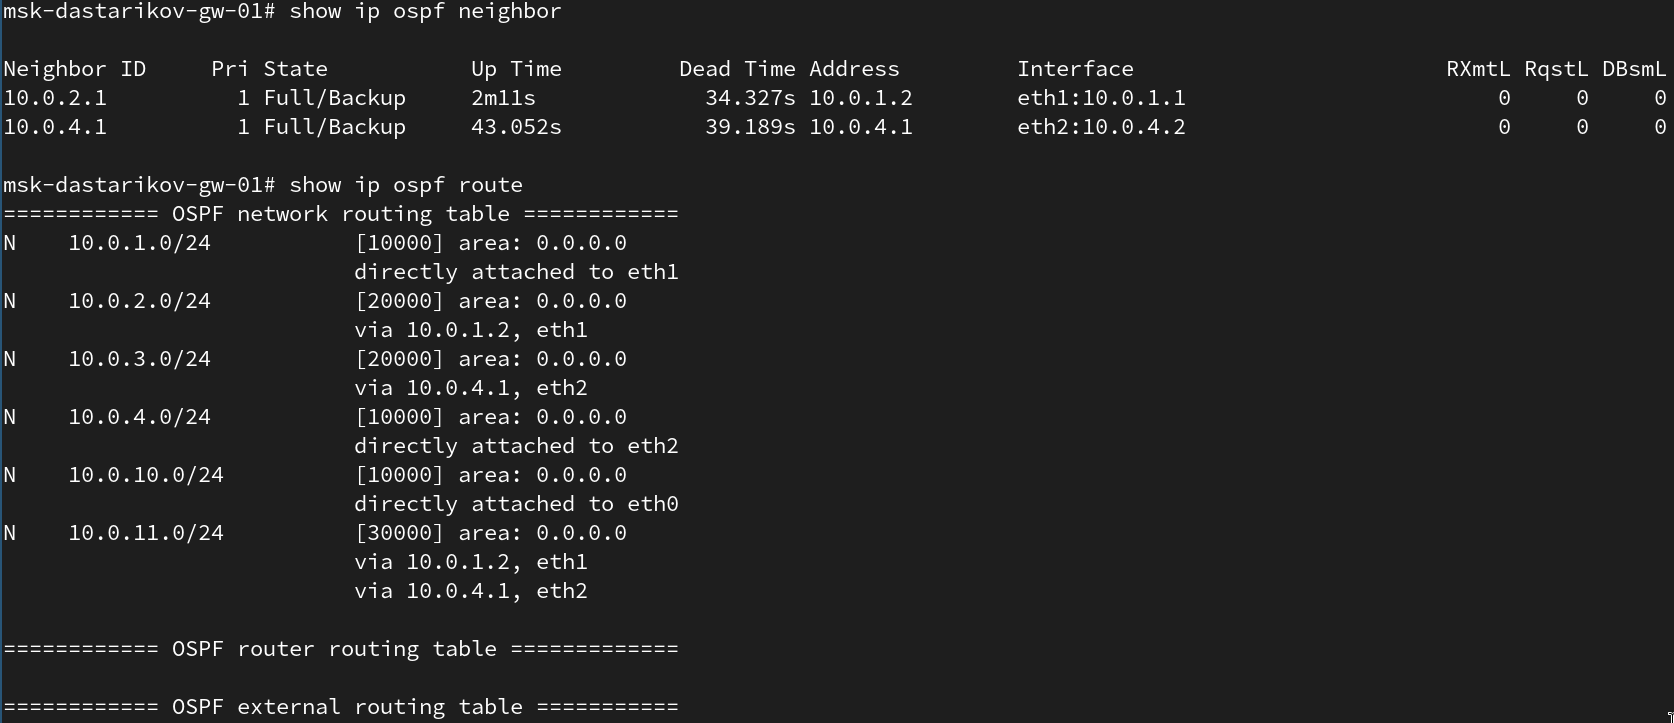
\includegraphics[width=0.8\textwidth]{../images/image46.png}
      \captionof{figure}{Просмотр таблицы маршрутизации протокола OSPFv2.}
\end{frame}

\begin{frame}
  \frametitle{Настройка динамической маршрутизации в сетях IPv4 и IPv6}
      \centering
      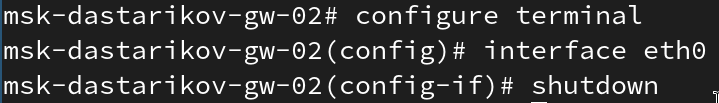
\includegraphics[width=0.8\textwidth]{../images/image47.png}
      \captionof{figure}{Отключение на маршрутизаторе \texttt{msk-dastarikov-gw-02} интерфейса \texttt{eth0}.}
\end{frame}

\begin{frame}
  \frametitle{Настройка динамической маршрутизации в сетях IPv4 и IPv6}
      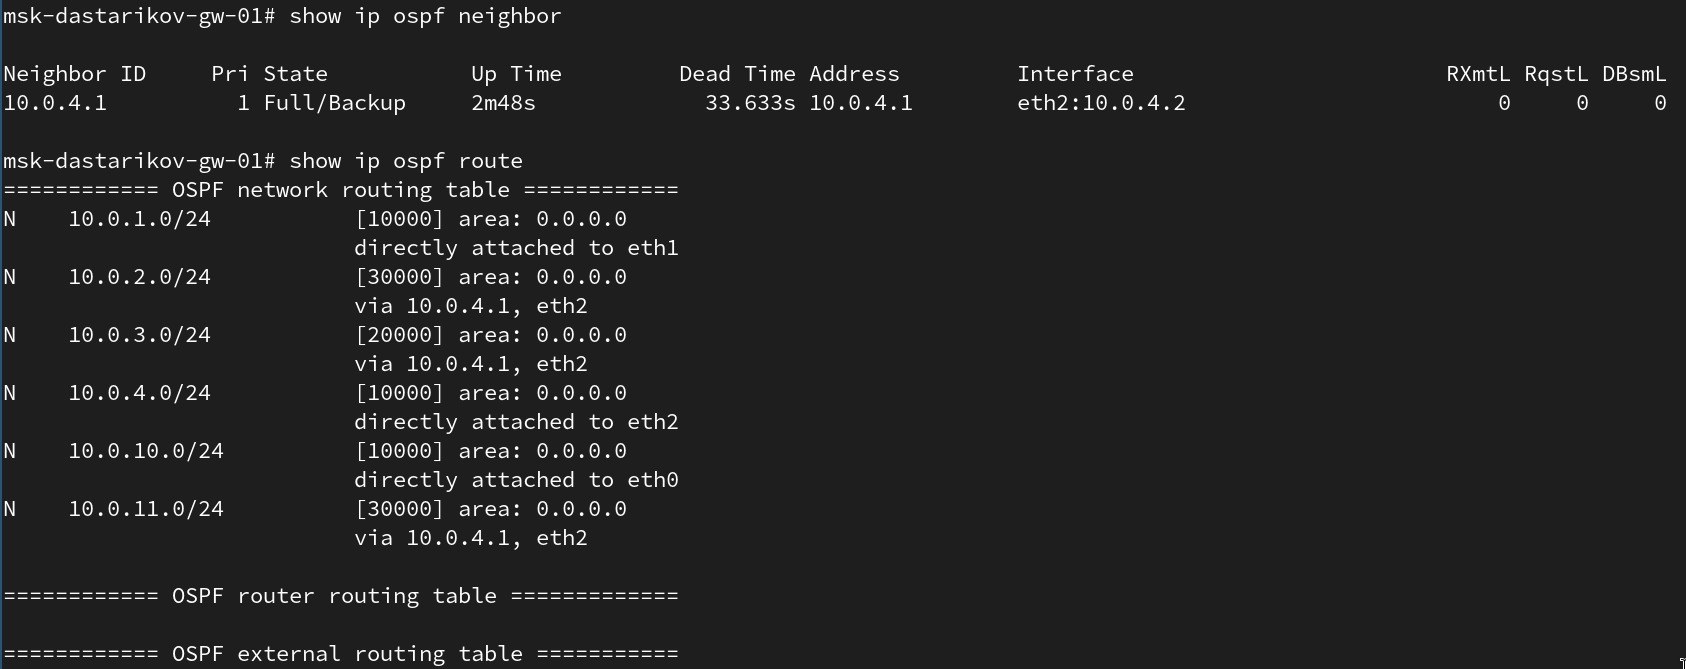
\includegraphics[width=0.8\textwidth]{../images/image49.png}
      \captionof{figure}{Просмотр таблицы маршрутизации протокола OSPFv2 после отключения интерфейса маршрутизатора.}
\end{frame}

\begin{frame}
  \frametitle{Настройка динамической маршрутизации в сетях IPv4 и IPv6}
      \centering
      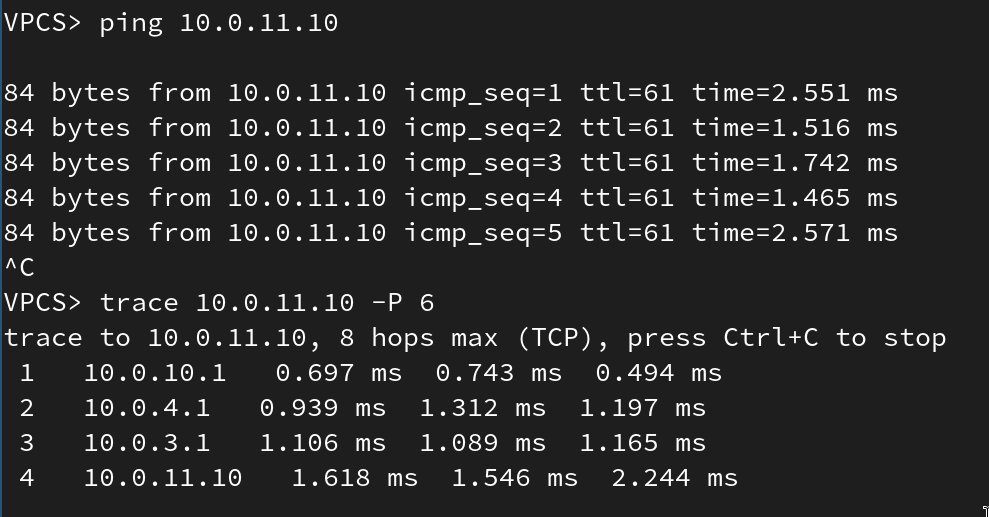
\includegraphics[width=0.8\textwidth]{../images/image51.png}
      \captionof{figure}{Отправка эхо-запроса с PC1 к PC2 после обновления маршрута.}
\end{frame}

\begin{frame}
  \frametitle{Настройка динамической маршрутизации в сетях IPv4 и IPv6}
      \centering
      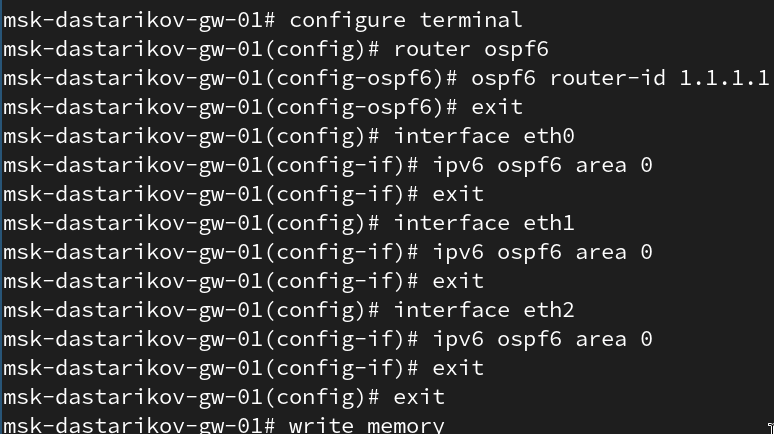
\includegraphics[width=0.8\textwidth]{../images/image53.png}
      \captionof{figure}{Настройка протокола OSPFv3 на маршрутизатору \texttt{gw-01}.}
\end{frame}

\begin{frame}
  \frametitle{Настройка динамической маршрутизации в сетях IPv4 и IPv6}
      \centering
      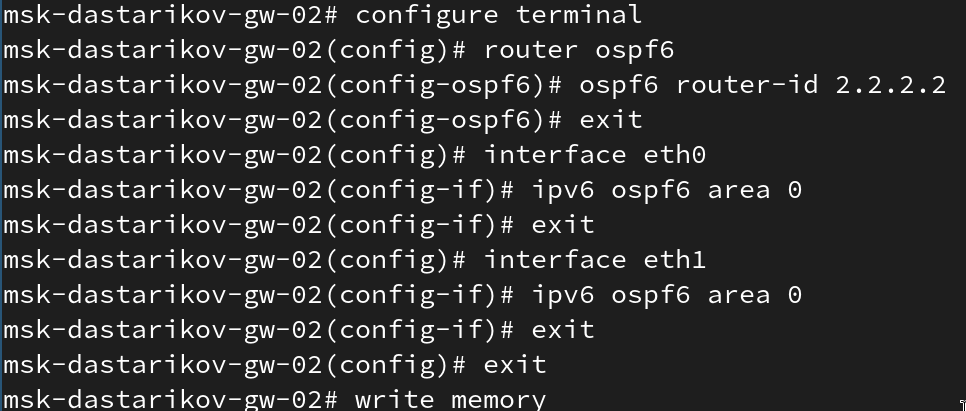
\includegraphics[width=0.8\textwidth]{../images/image54.png}
      \captionof{figure}{Настройка протокола OSPFv3 на маршрутизатору \texttt{gw-02}.}
\end{frame}

\begin{frame}
  \frametitle{Настройка динамической маршрутизации в сетях IPv4 и IPv6}
      \centering
      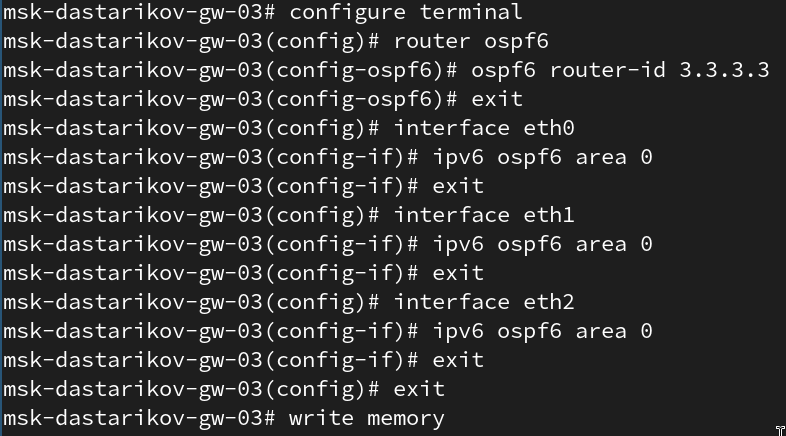
\includegraphics[width=0.8\textwidth]{../images/image55.png}
      \captionof{figure}{Настройка протокола OSPFv3 на маршрутизатору \texttt{gw-03}.}
\end{frame}

\begin{frame}
  \frametitle{Настройка динамической маршрутизации в сетях IPv4 и IPv6}
      \centering
      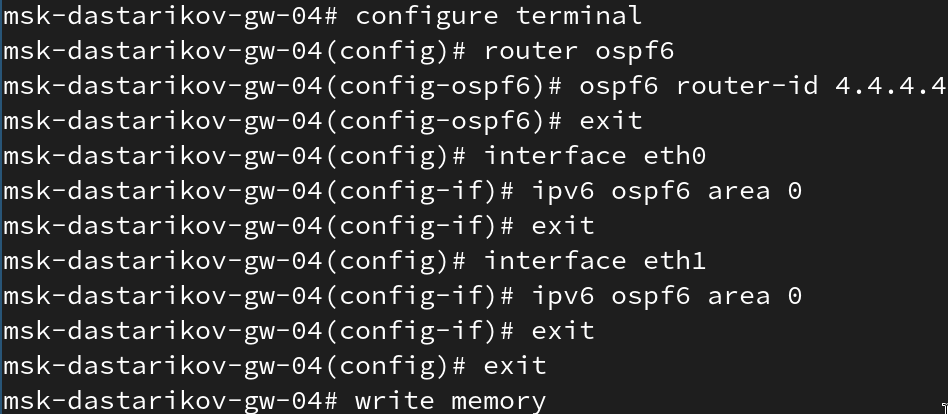
\includegraphics[width=0.8\textwidth]{../images/image56.png}
      \captionof{figure}{Настройка протокола OSPFv3 на маршрутизатору \texttt{gw-04}.}
\end{frame}

\begin{frame}
  \frametitle{Настройка динамической маршрутизации в сетях IPv4 и IPv6}
      \centering
      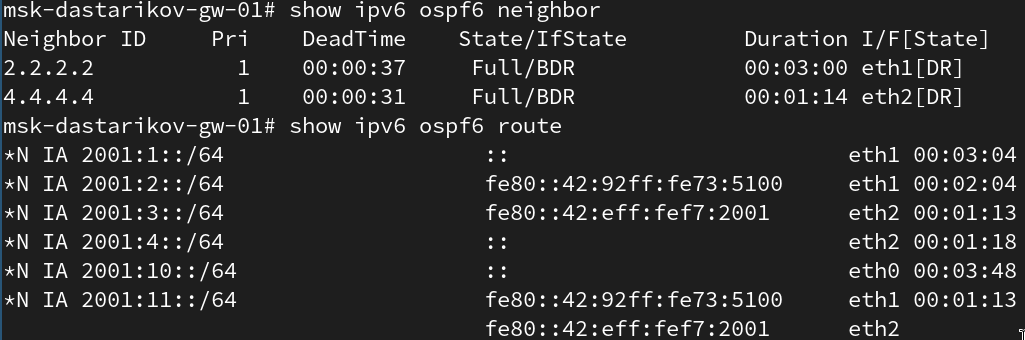
\includegraphics[width=0.8\textwidth]{../images/image58.png}
      \captionof{figure}{Проверка таблицы маршрутизации протокола OSPFv3.}
\end{frame}

\begin{frame}
  \frametitle{Настройка динамической маршрутизации в сетях IPv4 и IPv6}
      \centering
      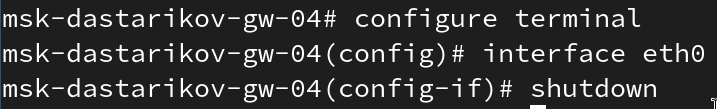
\includegraphics[width=0.8\textwidth]{../images/image59.png}
      \captionof{figure}{Отключение на маршрутизаторе \texttt{msk-dastarikov-gw-04} интерфейса \texttt{eth0}.}
\end{frame}

\begin{frame}
  \frametitle{Настройка динамической маршрутизации в сетях IPv4 и IPv6}
      \centering
      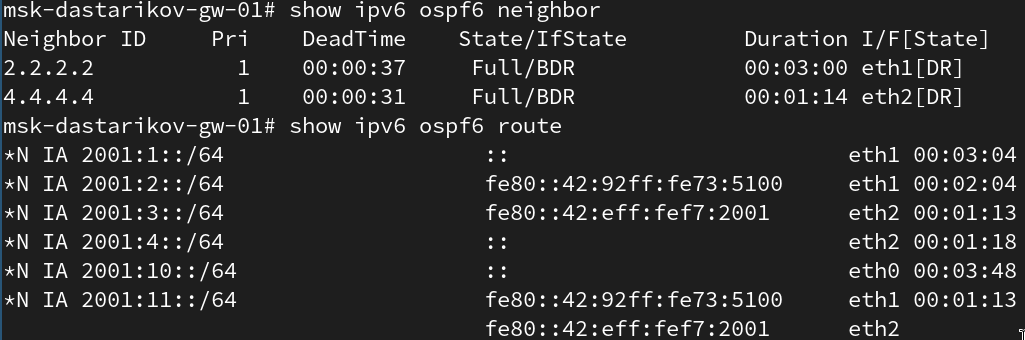
\includegraphics[width=0.8\textwidth]{../images/image58.png}
      \captionof{figure}{Проверка таблицы маршрутизации протокола OSPFv3 после отключения интерфейса маршрутизатора.}
\end{frame}

\begin{frame}
  \frametitle{Настройка динамической маршрутизации в сетях IPv4 и IPv6}
      \centering
      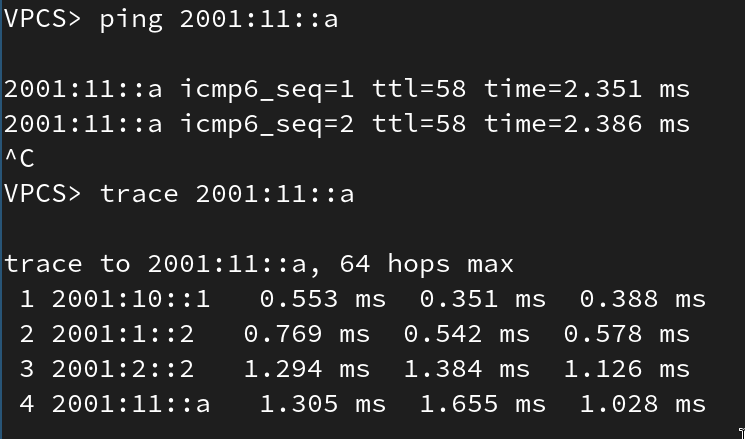
\includegraphics[width=0.8\textwidth]{../images/image61.png}
      \captionof{figure}{Отправка эхо-запроса с PC1 к PC2 по новому маршруту.}
\end{frame}



\begin{frame}
  \frametitle{Построение туннеля IPv6-IPv4}
  \begin{table}[]
    \centering
    \caption{Таблица адресации}
    \label{tab3}
    \begin{tabular}{|l|l|l|l|}
      \hline
      Устройство & Интерфейс & Адрес      & Шлюз по умолчанию \\ \hline
      R1         & eth0      & 1000::1/64 & –                 \\ \hline
      R1         & eth1      & 10.0.0.1/8 & –                 \\ \hline
      R1         & Tunnel0   & 1001::1/64 & –                 \\ \hline
      R2         & eth0      & 1002::1/64 & –                 \\ \hline
      R2         & eth1      & 20.0.0.2/8 & –                 \\ \hline
      R2         & Tunnel0   & 1001::2/64 & –                 \\ \hline
      R3         & eth0      & 10.0.0.2/8 & –                 \\ \hline
      R3         & eth1      & 20.0.0.1/8 & –                 \\ \hline
      PC1        & –         & 1000::a/64 & 1000::1           \\ \hline
      PC2        & –         & 1002::a/64 & 1002::1           \\ \hline
    \end{tabular}
  \end{table}
\end{frame}

\begin{frame}
  \frametitle{Построение туннеля IPv6-IPv4}
    \centering
    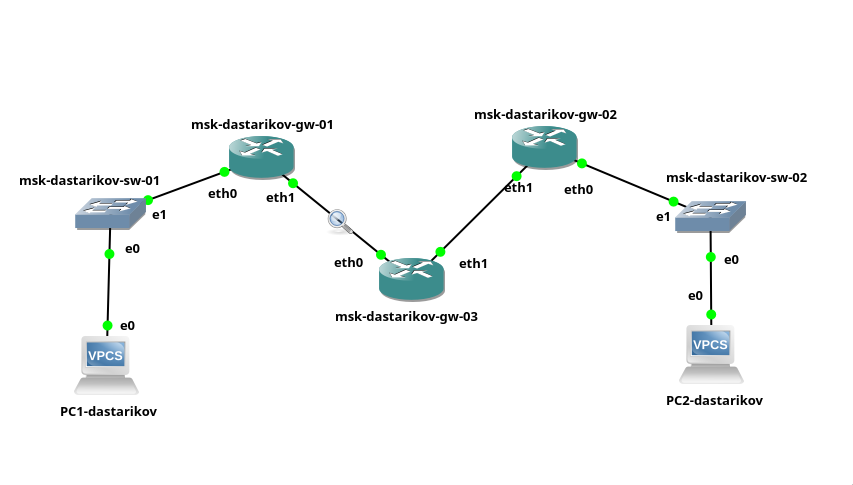
\includegraphics[width=0.8\textwidth]{../images/image83.png}
    \captionof{figure}{Топология сети.}
\end{frame}

\begin{frame}
  \frametitle{Построение туннеля IPv6-IPv4}
      \centering
      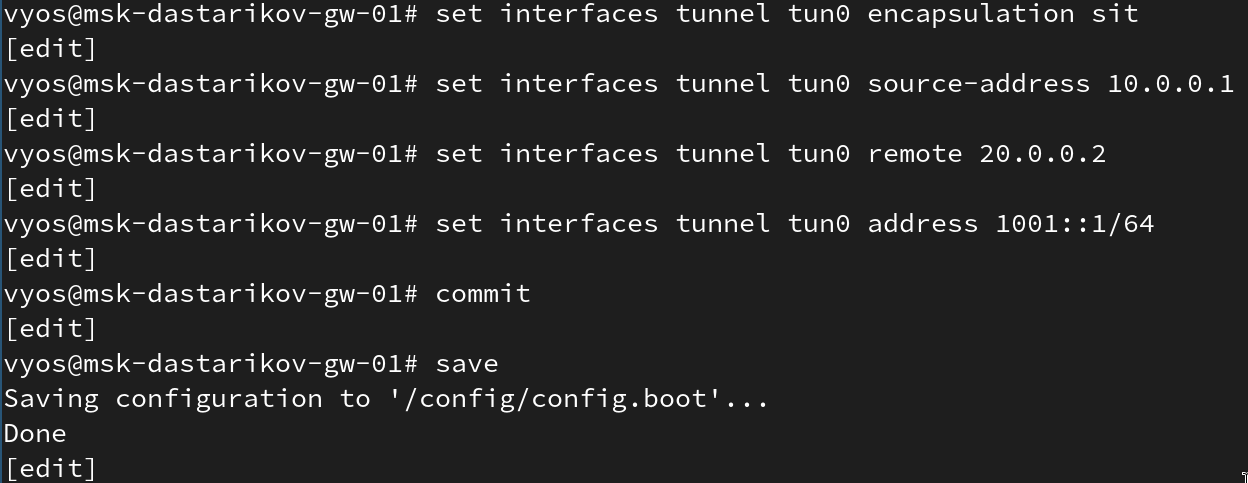
\includegraphics[width=0.8\textwidth]{../images/image70.png}
      \captionof{figure}{Настройка туннеля на маршрутизаторе \texttt{gw-01}.}
\end{frame}

\begin{frame}
  \frametitle{Построение туннеля IPv6-IPv4}
      \centering
      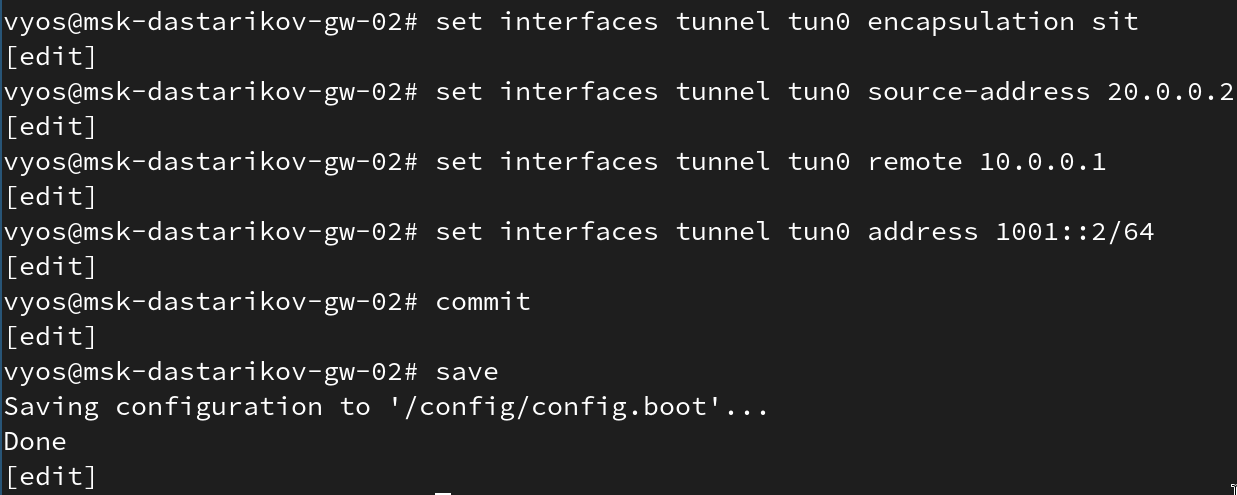
\includegraphics[width=0.8\textwidth]{../images/image71.png}
      \captionof{figure}{Настройка туннеля на маршрутизаторе \texttt{gw-02}.}
\end{frame}

\begin{frame}
  \frametitle{Построение туннеля IPv6-IPv4}
      \centering
      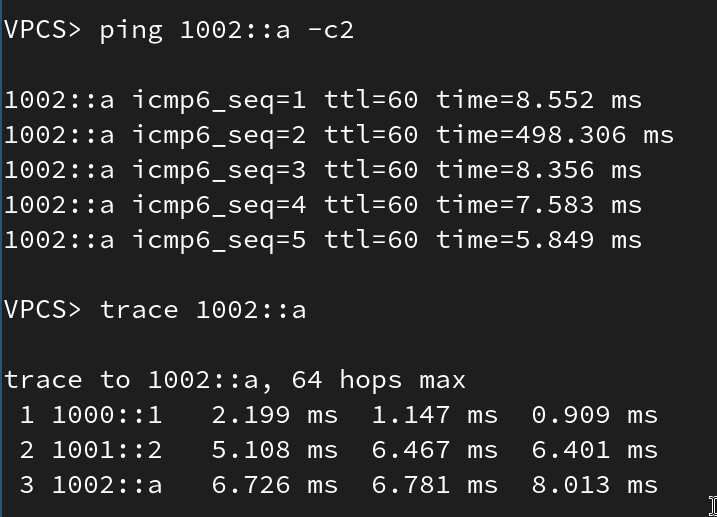
\includegraphics[width=0.8\textwidth]{../images/image79.png}
      \captionof{figure}{Проверка доступности PC2 с PC1.}
\end{frame}

\begin{frame}
  \frametitle{Построение туннеля IPv6-IPv4}
      \centering
      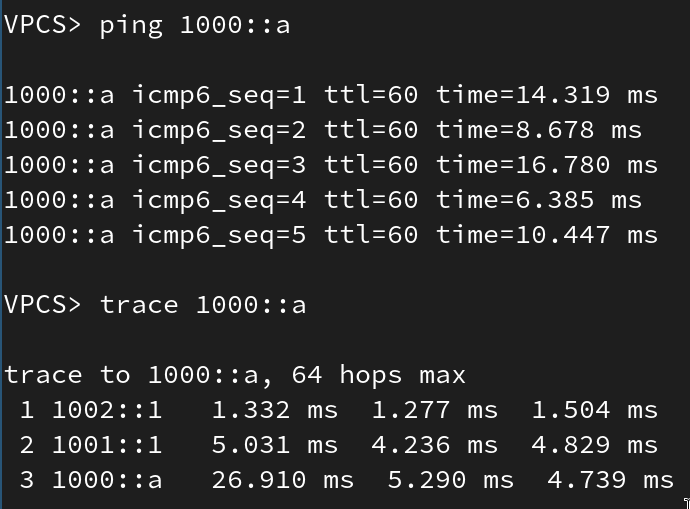
\includegraphics[width=0.8\textwidth]{../images/image80.png}
      \captionof{figure}{Проверка доступности PC1 с PC2.}
\end{frame}

\begin{frame}
  \frametitle{Построение туннеля IPv6-IPv4}
      \centering
      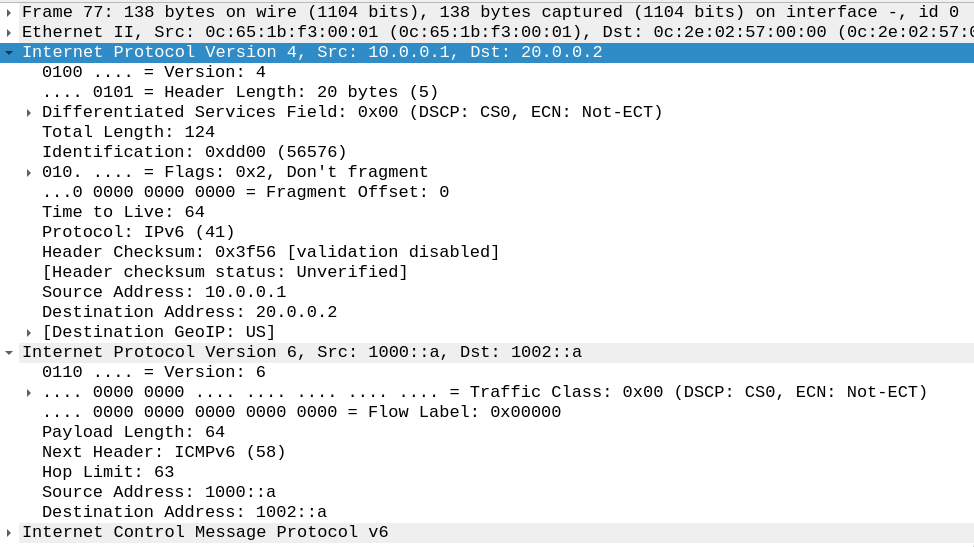
\includegraphics[width=0.8\textwidth]{../images/image81.png}
      \captionof{figure}{Перехваченый эхо-запрос с PC1 к PC2.}
\end{frame}

\begin{frame}
  \frametitle{Построение туннеля IPv6-IPv4}
      \centering
      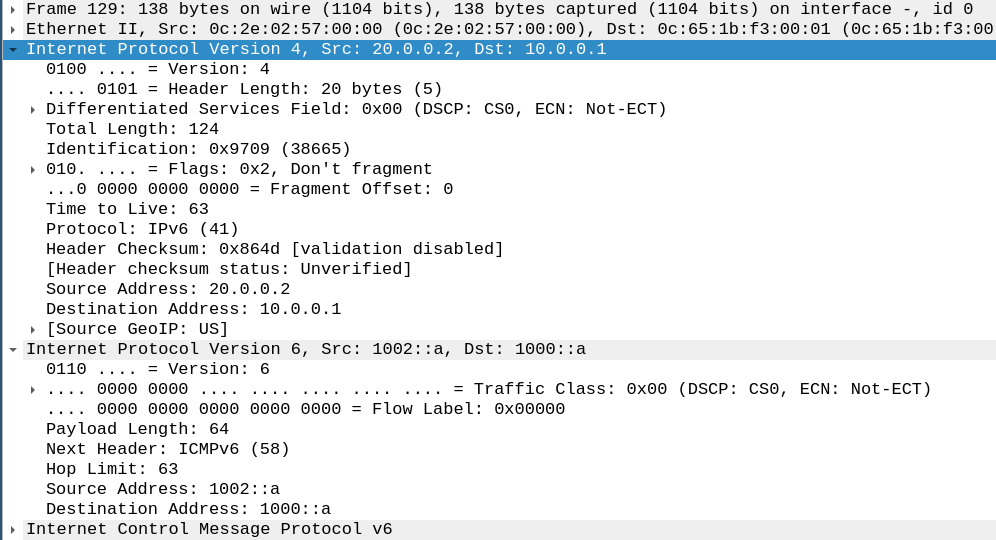
\includegraphics[width=0.8\textwidth]{../images/image82.png}
      \captionof{figure}{Перехваченый эхо-запрос с PC2 к PC1.}
\end{frame}

\begin{frame}
  \frametitle{Задание для самостоятельного выполнения}
    \centering
    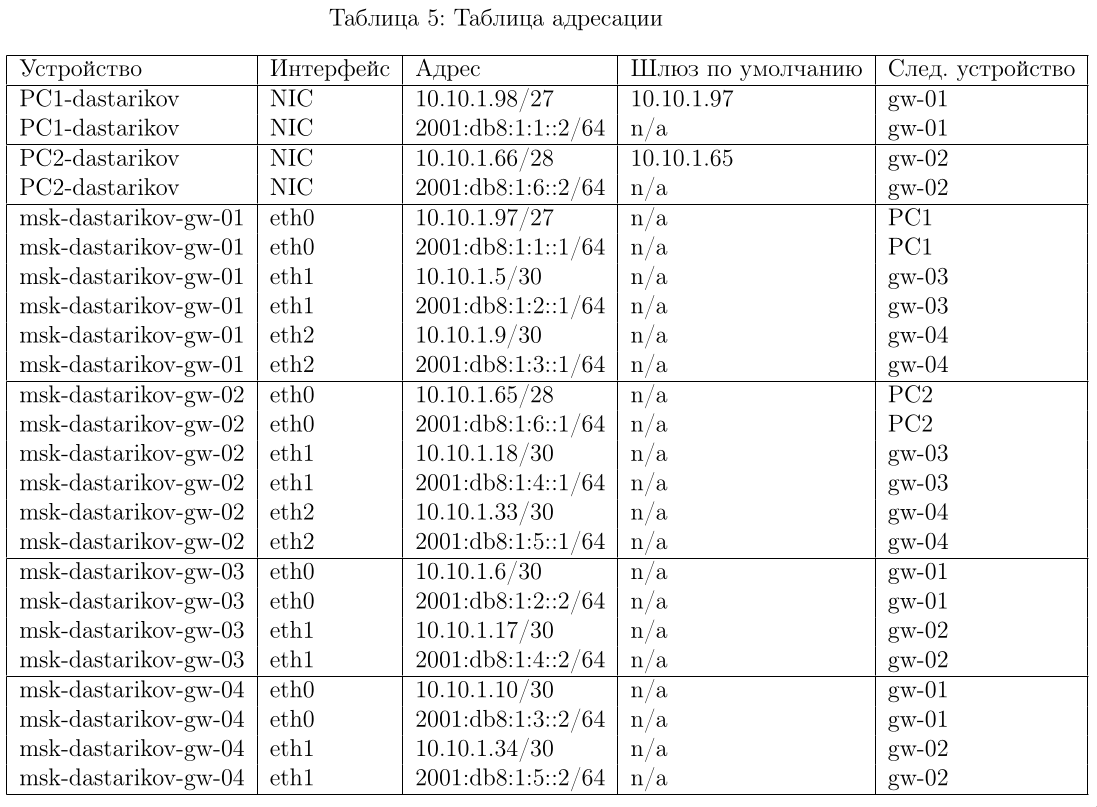
\includegraphics[width=0.8\textwidth]{../images/image_tab4.png}
    \captionof{figure}{Таблица адресации.}
\end{frame}

\begin{frame}
  \frametitle{Задание для самостоятельного выполнения}
    \centering
    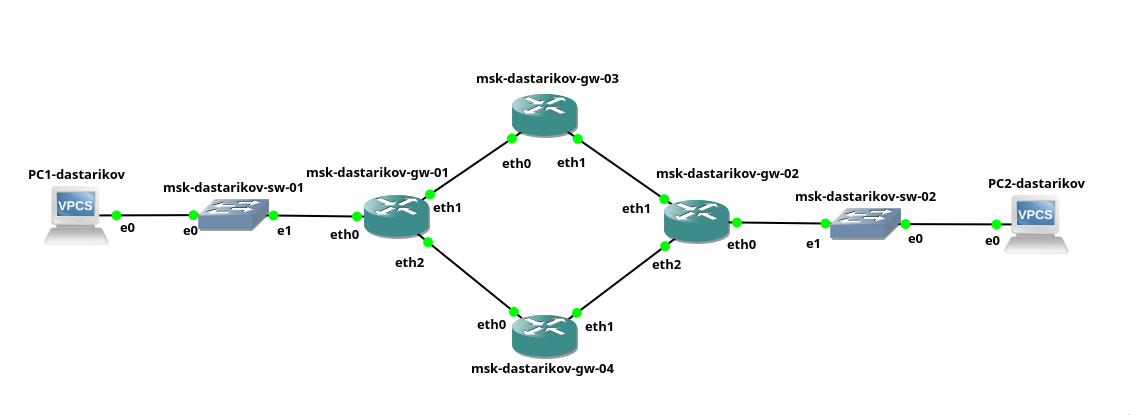
\includegraphics[width=0.8\textwidth]{../images/image133.png}
    \captionof{figure}{Топология сети.}
\end{frame}

\begin{frame}
  \frametitle{Задание для самостоятельного выполнения}
  \begin{table}[]
    \centering
    \caption{Таблица адресов сетей}
    \label{tab6}
    \begin{tabular}{lll}
      Устройства  & Сеть IPv4     & Сеть IPv6         \\
      PC1–gw-01   & 10.10.1.96/27 & 2001:db8:1:1::/64 \\
      PC2–gw-02   & 10.10.1.64/28 & 2001:db8:1:6::/64 \\
      gw-01–gw-03 & 10.10.1.4/30  & 2001:db8:1:2::/64 \\
      gw-02–gw-04 & 10.10.1.8/30  & 2001:db8:1:3::/64 \\
      gw-03–gw-02 & 10.10.1.16/30 & 2001:db8:1:4::/64 \\
      gw-04–gw-02 & 10.10.1.32/30 & 2001:db8:1:5::/64
    \end{tabular}
  \end{table}
\end{frame}

\begin{frame}
  \frametitle{Задание для самостоятельного выполнения}
      \centering
      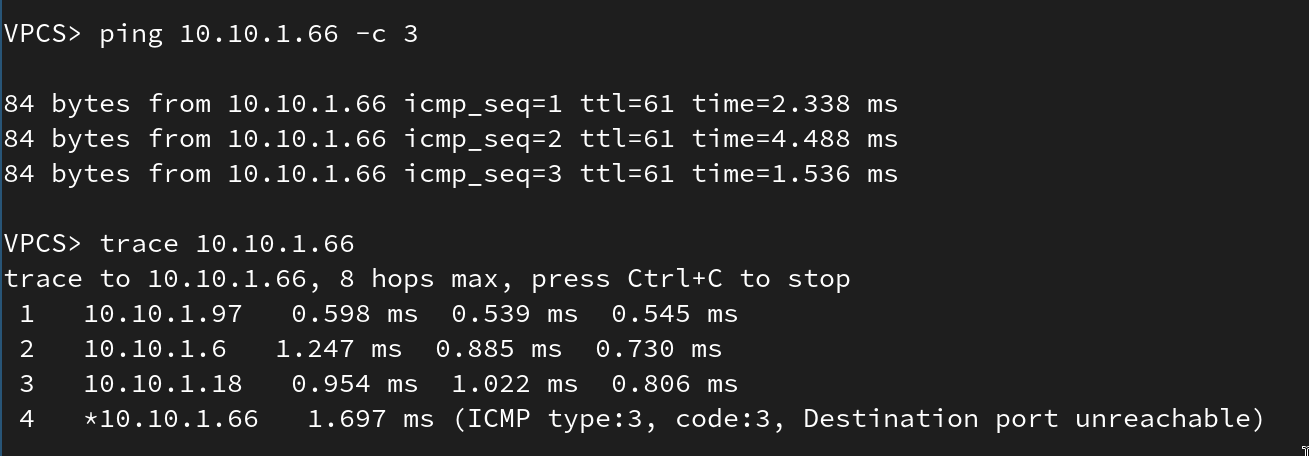
\includegraphics[width=0.8\textwidth]{../images/image102.png}
      \captionof{figure}{Проверка доступности PC1 с PC2.}
\end{frame}

\begin{frame}
  \frametitle{Задание для самостоятельного выполнения}
      \centering
      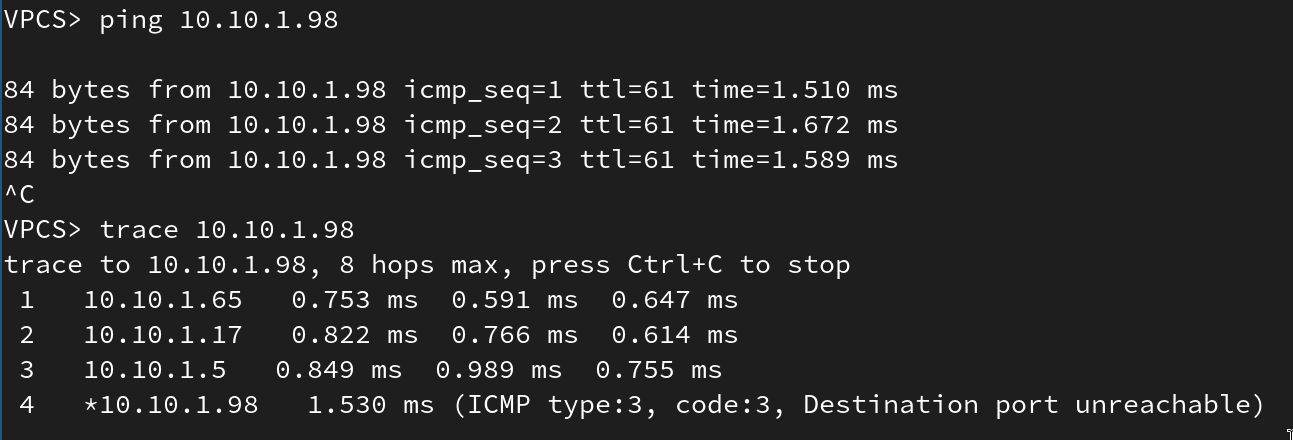
\includegraphics[width=0.8\textwidth]{../images/image103.png}
      \captionof{figure}{Проверка доступности PC2 с PC1.}
\end{frame}

\begin{frame}
  \frametitle{Задание для самостоятельного выполнения}
      \centering
      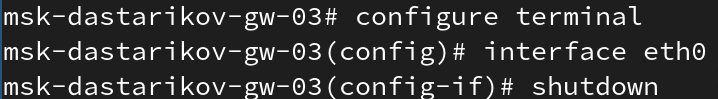
\includegraphics[width=0.8\textwidth]{../images/image104.png}
      \captionof{figure}{Отключение на маршрутизаторе \texttt{msk-dastarikov-gw-03} интерфейса \texttt{eth0}.}
\end{frame}

\begin{frame}
  \frametitle{Задание для самостоятельного выполнения}
      \centering
      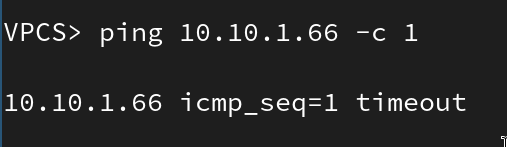
\includegraphics[width=0.8\textwidth]{../images/image105.png}
      \captionof{figure}{Отсутствие доступа после отключения интерфейса.}
\end{frame}

\begin{frame}
  \frametitle{Задание для самостоятельного выполнения}
      \centering
      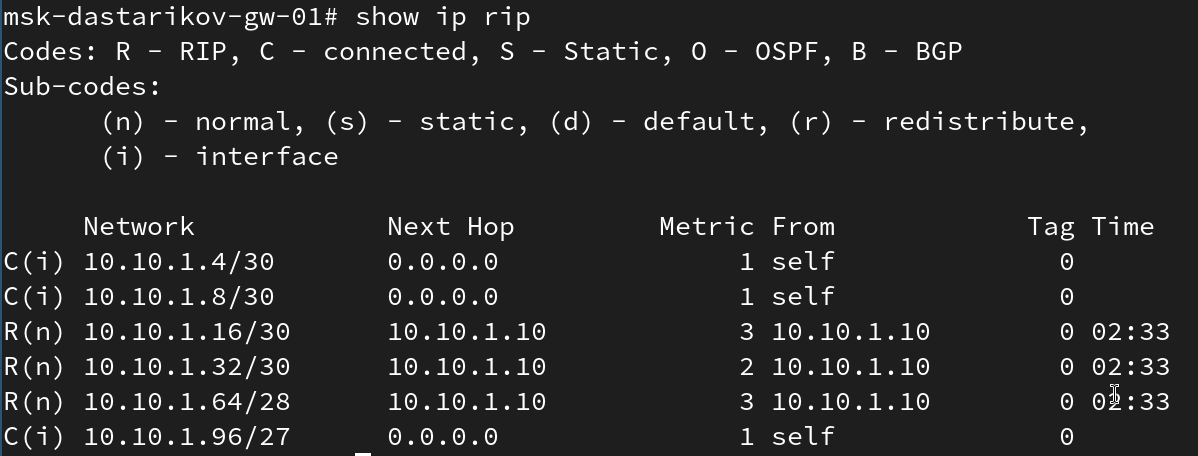
\includegraphics[width=0.8\textwidth]{../images/image106.png}
      \captionof{figure}{Просмотр таблицы маршрутизации RIP после отключения интерфейса.}
\end{frame}

\begin{frame}
  \frametitle{Задание для самостоятельного выполнения}
      \centering
      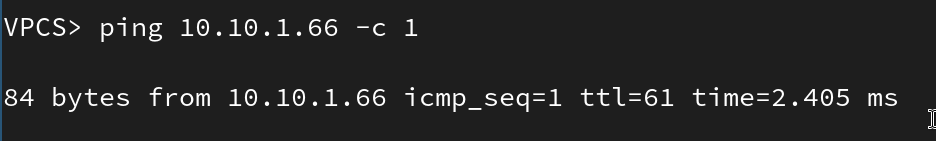
\includegraphics[width=0.8\textwidth]{../images/image107.png}
      \captionof{figure}{Восстановление доступа после отключения интерфейса.}
\end{frame}

\begin{frame}
  \frametitle{Задание для самостоятельного выполнения}
      \centering
      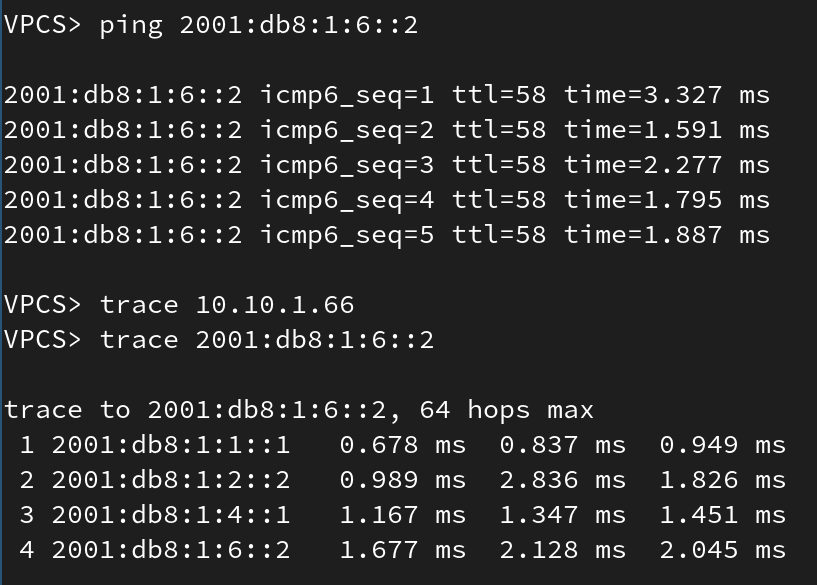
\includegraphics[width=0.8\textwidth]{../images/image112.png}
      \captionof{figure}{Проверка доступности PC1 с PC2.}
\end{frame}

\begin{frame}
  \frametitle{Задание для самостоятельного выполнения}
      \centering
      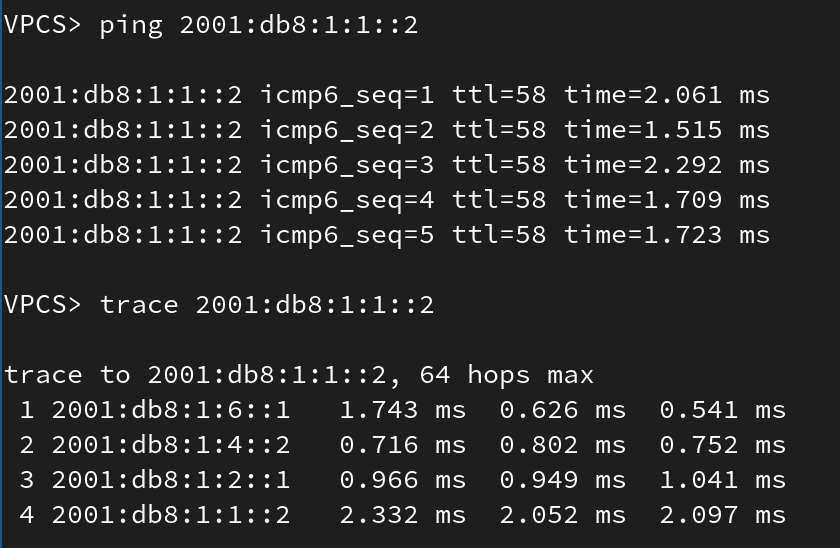
\includegraphics[width=0.8\textwidth]{../images/image113.png}
      \captionof{figure}{Проверка доступности PC2 с PC1.}
\end{frame}

\begin{frame}
  \frametitle{Задание для самостоятельного выполнения}
      \centering
      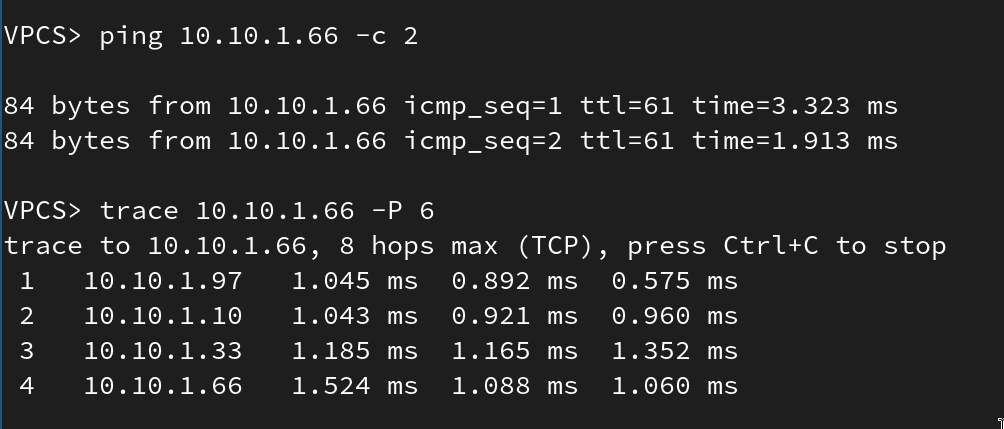
\includegraphics[width=0.8\textwidth]{../images/image121.png}
      \captionof{figure}{Проверка доступности PC1 с PC2.}
\end{frame}

\begin{frame}
  \frametitle{Задание для самостоятельного выполнения}
      \centering
      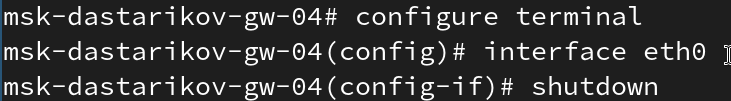
\includegraphics[width=0.8\textwidth]{../images/image123.png}
      \captionof{figure}{Отключение на маршрутизаторе \texttt{msk-dastarikov-gw-04} интерфейса \texttt{eth0}.}
\end{frame}

\begin{frame}
  \frametitle{Задание для самостоятельного выполнения}
      \centering
      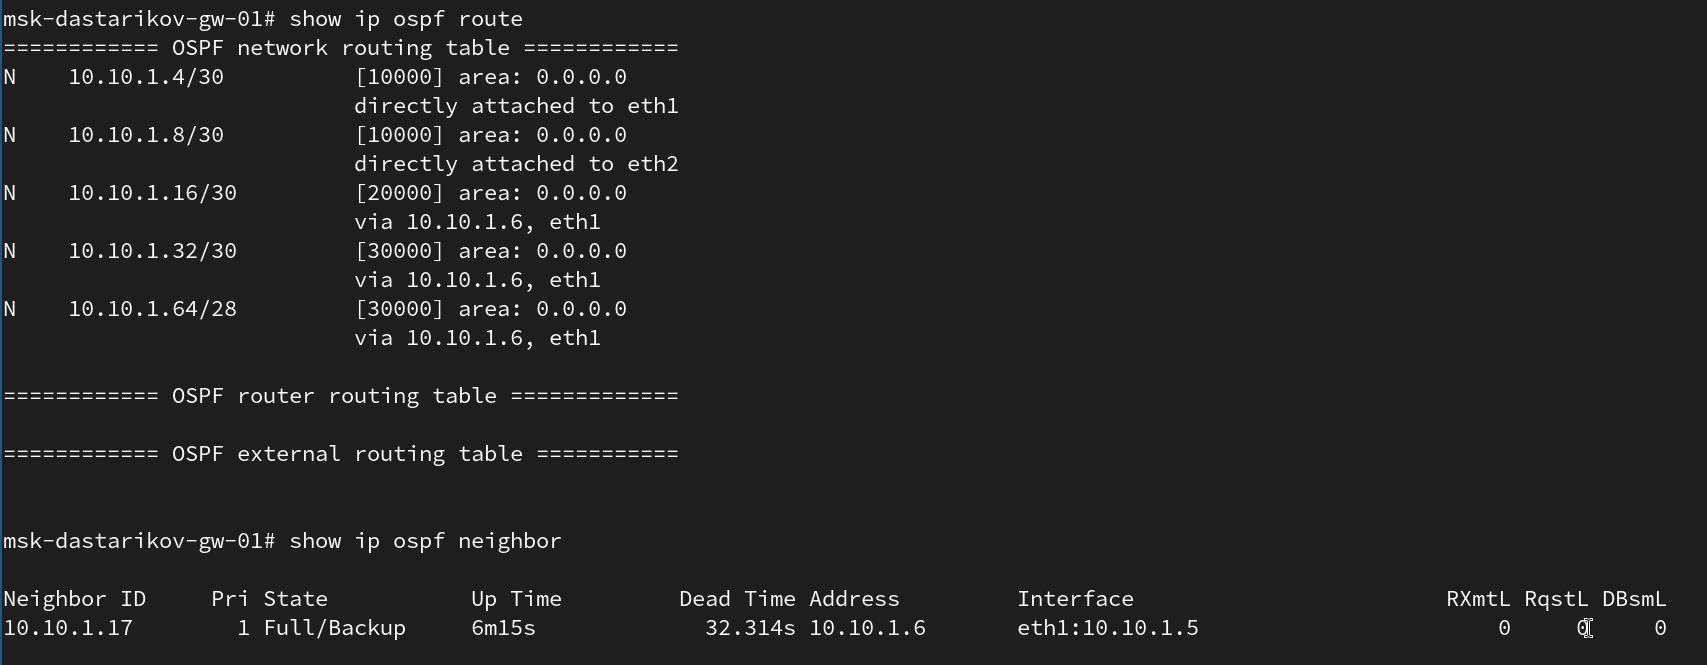
\includegraphics[width=0.8\textwidth]{../images/image125.png}
      \captionof{figure}{Просмотр таблицы маршрутизации OSPF после отключения интерфейса.}
\end{frame}

\begin{frame}
  \frametitle{Задание для самостоятельного выполнения}
      \centering
      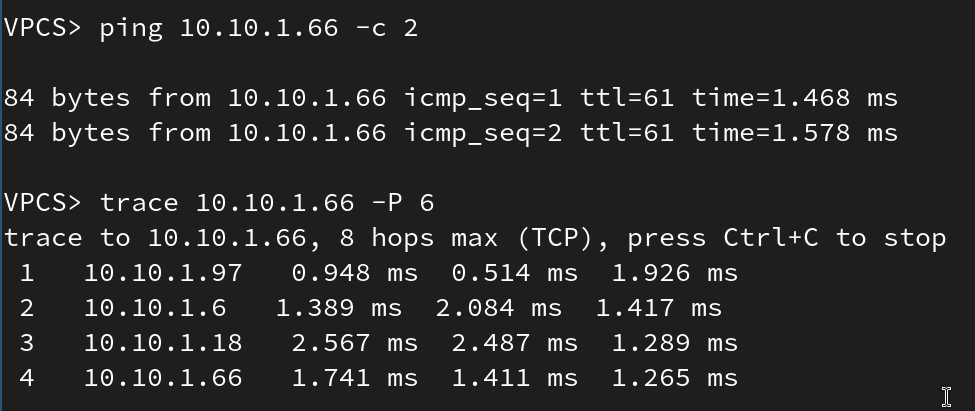
\includegraphics[width=0.8\textwidth]{../images/image124.png}
      \captionof{figure}{Восстановление доступа после отключения интерфейса.}
\end{frame}

\begin{frame}
  \frametitle{Задание для самостоятельного выполнения}
      \centering
      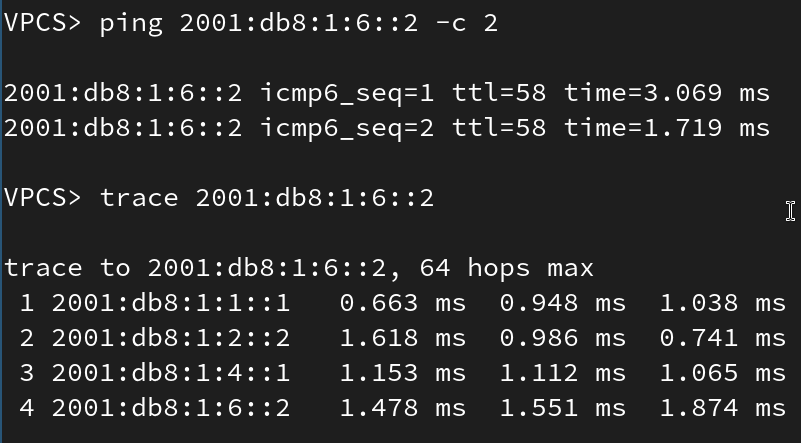
\includegraphics[width=0.8\textwidth]{../images/image129.png}
      \captionof{figure}{Проверка доступности PC1 с PC2.}
\end{frame}

\begin{frame}
  \frametitle{Задание для самостоятельного выполнения}
      \centering
      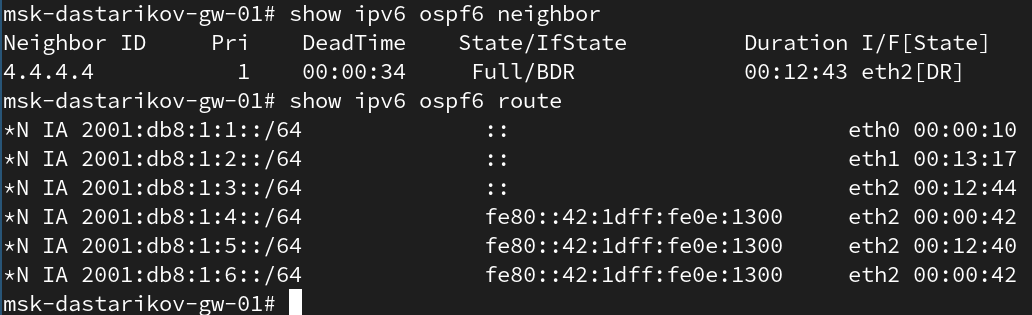
\includegraphics[width=0.8\textwidth]{../images/image132.png}
      \captionof{figure}{Просмотр таблицы маршрутизации OSPFv3 после отключения интерфейса.}
\end{frame}

\begin{frame}
  \frametitle{Задание для самостоятельного выполнения}
      \centering
      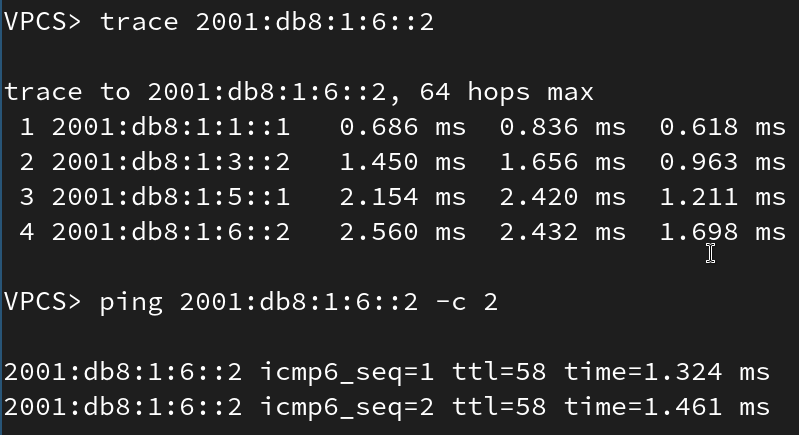
\includegraphics[width=0.8\textwidth]{../images/image131.png}
      \captionof{figure}{Восстановление доступа после отключения интерфейса.}
\end{frame}

\begin{frame}
  \frametitle{Выводы}
  \begin{itemize}
  \item В результате выполнения лабораторной работы изучили принципы маршрутизации в IPv4- и IPv6-сетях и принципы настройки сетевого оборудования
  \item Самостоятельно настроили сеть с двойным стеком IPv4 и IPv6, динамической маршрутизацией для протоколов RIP и OSPF и проверили соединения и маршруты
  \end{itemize}
\end{frame}
\end{document}
